\documentclass[12pt,letterpaper]{article}
\usepackage[utf8]{inputenc}
\usepackage{amsmath}
\usepackage{amsfonts}
\usepackage{amssymb}
\usepackage{listings}
\usepackage{hyperref}
\usepackage{color}
\usepackage{graphicx} %for pngs
\usepackage[left=1in,right=1in,top=1in,bottom=1in]{geometry}
\author{Nathaniel Beaver}
\title{A description of software for searchable math and physics equations, identities, and definitions.}
\begin{document}

\maketitle

\section{Motivation}

Physicsists and mathematicians use equations a lot. However, they tend to refer to books or websites when looking them up, both of which suffer from fairly severe flaws, such as inability to search effectively by the structure of the equation.

\section{Use case}

Suppose I want to look up boundary conditions for an electric field to include in a paper I am writing.

\subsection{Print resources.}

Most physicists will reach for their trusty E\&M books in this case.

In the 2nd edition of David J. Griffiths' ``Introduction to Electrodynamis'', for example, a search of the index for ``Boundary conditions'' gives these equations (in SI units) on page 313:
\begin{align*}
D_{1_\bot} - D_{2_\bot} &= \sigma_f \\
E_{1_\parallel} - E_{1_\parallel} &= 0
\end{align*}

The 3rd edition of John David Jackson's ``Classical Electrodynamics'' also uses SI units, and a quick check of the index gives:
\begin{align*}
(\mathbf{D}_1 - \mathbf{D}_2)\cdot \mathbf{n} &= \sigma \\
n \times (\mathbf{E}_2 - \mathbf{E}_1) &= 0
\end{align*}

The drawback is that these equations have to be manually typed up for use in a \LaTeX\ document or word processing software, a laborious process even for relatively short equations. Ebooks and PDF files do not solve this problem.

\subsection{Electronic resources.}

For quick and dirty information finding, Google works well. Let's see what the top results are.
\url{https://www.google.com/search?q=electric+field+boundary+conditions}

The first result, as of \today, is
\url{http://farside.ph.utexas.edu/teaching/em/lectures/node59.html}
. This website explains their origin from Gauss's Law and gives the equations as embedded png images:

\begin{center}
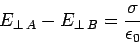
\includegraphics[scale=0.5]{img1337.png}

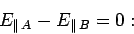
\includegraphics[scale=0.5]{img1344.png}
\end{center}

The second result is here: \url{http://www.antenna-theory.com/tutorial/electromagnetics/electric-field-boundary-conditions.php}

This page distinguishes between a charged/uncharged surface and uses different notation and units. They also use images, gif in this case (although I converted them to png for inclusion in this document):
\begin{center}
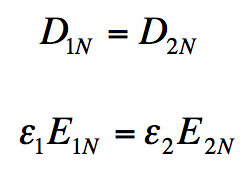
\includegraphics[scale=0.3]{normalDequal.png}
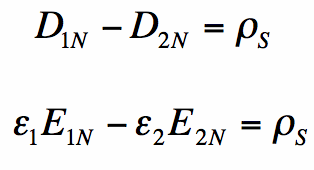
\includegraphics[scale=0.3]{normalEfieldWithCharge.png}
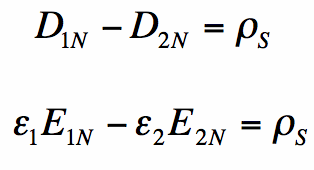
\includegraphics[scale=0.3]{normalEfieldWithCharge.png}
\end{center}

Note that already there is considerable variation in notation. Furthermore, neither site includes any equations which can be parsed or modified without performing optical character recognition on the images; they are heavily read-only.

What about Wikipedia?

\url{https://en.wikipedia.org/wiki/Interface_conditions_for_electromagnetic_fields}

This is the relevant equation.

\begin{center}
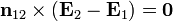
\includegraphics[scale=0.5]{wikipedia1.png}

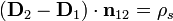
\includegraphics[scale=0.5]{wikipedia2.png}
\end{center}

Fortunately, there is embedded \LaTeX\ markup available under ``Edit Source''.

\begin{verbatim}
:<math>\mathbf{n}_{12} \times (\mathbf{E}_2 - \mathbf{E}_1)  = \mathbf{0} </math>

:<math>(\mathbf{D}_2 - \mathbf{D}_1) \cdot \mathbf{n}_{12} = \rho_{s} </math>
\end{verbatim}

This will only be sufficient if:
\begin{enumerate}
\item I want \LaTeX\ markup.
\item the Wikipedia editor uses the \LaTeX\ markup correctly.
\item the Wikipedia markup uses the same symbols and units system.
\end{enumerate}

\section{The problem.}

Both the print and electronic resources have a number of deficiencies. In particular,
\begin{itemize}
\item There is no reliable standard for representation of variables, even for the simplest and most common equations. Sometimes a surface charge is $\sigma$, sometimes it is $\sigma_f$, and sometimes it is $\rho_s$.
\item There are \href{https://en.wikipedia.org/wiki/Systems_of_units}{many units systems in use in the sciences}, several of which are popular enough to include in, say, the \href{http://lammps.sandia.gov/doc/units.html}{software of a given subfield}, and even if everyone were to standardize tomorrow there is centuries of scholarly literature that is expressed in different units. One of the most common examples is the differing forms of equations for SI (MKSA) and Gaussian (cgs) systems. There are valid arguments for using either system, or using the so-called ``natural units''. Converting between these systems, however, is tedious, and people should not have to spend much time on it.
\item In much the same way as there are many unit systems, there are many equally valid \href{https://en.wikipedia.org/wiki/Gauge_fixing}{choices of gauge} in electrodynamics and a \href{https://en.wikipedia.org/wiki/Tensor_notation}{proliferation of tensor notations}.
\item No print or electronic resource is free from errors, and not everyone checks the errata page.
\end{itemize}

Together, these problems can make what should be simple tasks into a chore. There is frequently unnecessary friction, for example, in using results from two different papers or collaborating with a colleague who uses a different unit system. And how many scholars have lost hours of work have been lost by writing a paper with one choice of symbols and units and having to change them all for a journal submission?

\section{What the solution should look like.}

Instead of trying to solve these problems by convincing everyone to use the same units, gauges, and symbols, it is much more sane to leverage the ability of machines to do busywork.

An electronic database of equations with the relevant information could easily translate between any system of units, and could produce output suitable for any software, regardless of whether it is intended for use in a Fortran program, a \LaTeX\ document, or a web browser.

If a transformation between these forms is non-trivial, the best thing is simply to have a human provide the input and store them both, and make them easy to find later. Rather than attempting to find the ``one true form'' of the equation, it should simply associate various useful formats.

Furthermore, it should take free-form input queries that would outpace any web search or paper index. This could include items like common names (``Maxwell equations''), units of variables (all equations with the left side in units of force), and even algebraic forms (all equations of the form \verb|a x^2 + b x + c|). Given sufficient heuristics and metadata (much of which will, admittedly, have to be entered manually), this is a solvable problem.

Finally, it should be personal and collaborative. It should be easy to import the standard equations, but most people have specific, personalized needs and collaborate with a relatively small group of people, so this software should reflect that.

\section{Features}

\label{features}

A satisfactory electronic equation reference document would:

\begin{itemize}
\item Store equation database locally (network connectivity not required).
\item Provide a means to write explanatory text for symbols or sub-expressions in the relevant equations, which most texts do anyway as a matter of course. For example, $\vec{L} = I \vec{\omega}$, where $\vec{L}$ is angular momentum, $I$ is the moment of inertia, and $\vec{\omega}$ is the angular velocity.
\item Store representations in at least one format of a variety of options (\LaTeX, MathML, OpenMath, etc.) as well as a way to add more specific forms. For example, one might be a \LaTeX\ expression with the vector quantities having arrows like this $\vec{r}$, and another with vector quantities bolded like this $\mathbf{r}$.
\item Provide the ability to optionally store and access other formats (e.g. Mathematica, MS Word, Matlab code, Fortran code, C code etc.)
\item Call existing software to convert between representations so that not everything has to be converted manually. This falls into two categories:
\begin{enumerate}
\item Conversions that are essentially just formatting conversions. For example, while \LaTeX and MathML have some very apparent differences, they both require only enough information to typeset an equation, not actually evaluate it. The automatically generated markup could subsequently be tweaked by hand.
\item Conversions from a typesetting or markup language like \LaTeX or MathML to an expression that can actually be evaluated; one that you can plug in numbers and get an answer. Some equations are simple enough that a conversion to, say, C code is trivial -- something just using trig, exponents, and arithmetic functions, for example. Others will be sufficiently abstract as to require manual conversion or avoiding a computable format at all. (Alternately, a link to some remotely hosted code may be in order; \hyperref[linking]{see below}.) Incidentally, Stephen Wolfram had this \href{http://www.stephenwolfram.com/publications/recent/mathml/mathml1.html} {to say} about this kind of conversion.
\begin{quote}
Unlike with ordinary human natural language, it is actually possible to take a very close approximation to familiar mathematical notation, and have a computer systematically understand it. That's one of the big things that we did about five years ago in the third version of Mathematica. And at least a little of what we learned from doing that actually made its way into the specification of MathML. 
\end{quote}
\end{enumerate}
\item Perform queries based on popular names, form of equations, related equations, commonly used symbols.
\item Perform queries based on similarity to a given input.
\item Provide the option to perform simple substitutions (so a query for $a+b^2$ could return an equation stored as $x+y^2$, and one could specify substitution rules so that it outputs $m + n^2$)
\item Provide the option to search for algebraically equivalent forms (e.g. $a(b+c)$ could return $a b + a c$). Note that this would only work for equations that had unambiguous computable forms provided, so that the software could call, e.g. Sage, Maxima, or Mathematica to determine whether or not the forms are algebraically equivalent. MathML or \LaTeX compilers will happily typeset algebraically ambiguous or uncomputable gibberish.
\item Provide the option to search for algebraically equivalent forms with simple substitutions (e.g.  $a(b+c)$ could return $ x y + x z$)
\item Provide the option to choose units system, so that a single equation would have both cgs and SI forms available, for example.
\item Allow extensions to specify new unit systems or gauges.
\item Link to internal and external references (refer to another equation in the same database, jump to a specified page of a local or remote PDF or ebook, standard html-style links to  urls of relevant websites or source code implementations, digital object identifiers, bibtex references, etc.) 
\end{itemize}

\section{Some objections.}

\label{linking}

\subsection{There's more to physics and math than equations, you know.}

Yes, and people did math for centuries without nice modern algebraic notation, but equations do provide a very lovely and compact way to represent relationships between variables.

Once we've got an easy and reliable way to find the equations we want, we can spend more time reasoning about whether the equation is applicable, what approximations to make, and what the physical interpretation is and how that squares with experiment and physical intuition.

\subsection{Equations without context are dangerous and people will use them when they are not really applicable or assume what they are trying to prove, i.e.\ use circular reasoning.}

A valid concern, which is why it's important to write explanatory text about each symbol and link to more complete discussions.

In any case, people already use equations when they aren't applicable, and this is generally because they don't want to put in the effort to look up the context of the equation. Properly used, this software could help mitigate this problem.

\subsection{Why ``equations'' and not ``expressions'' or ``formulas''?}

This is just a nomenclature thing.

I assume that this software could work for mathematical expressions in general, identities, approximations, chemical formulas, etc. Most of the time, though, we need to know about relationships between variables, so ``equations'' are what most people think of and use regularly.

\subsection{Is it really so much work to use a web search or a book index?}

Yes.

Try doing a \href{https://www.google.com/search?q=%22L+%3D+r+%C3%97+P%22&oq=%22L+%3D+r+%C3%97+P%22}{Google search for $L = r \times p$}. \href{http://symbolab.com/search?origin=suggestion&query=L%3Dr%5Ctimes%20p}{Symbolab works somewhat better} for this, as does \href{https://www.google.com/search?&q=%22L+%3D+r+%5Ctimes+P%22&oq=%22L+%3D+r+%5Ctimes+P%22
}{searching for likely \LaTeX markup}.

This is just a simple example of hard it is to find even a basic equation with relatively few ways to express it.

%TODO add more examples explaining how badly things are broken and why this needs to change

As for books, if you can get everything you need from one book, great. The ones I need are generally scattered across several books and journal articles, none of which have the same notation and only some of which have good indices.

\subsection{Surely there are people already working on this, or something similar?}

There are some
\href{http://symbolab.com/}{interesting} \href{http://latexsearch.com/}{websites} \href{http://www.dessci.com/en/reference/searching/math-searching.htm}{out}
\href{http://www.equationsheet.com/}{there},
but they're more about searching existing websites and scholarly literature and don't accomplish more than a few of the \hyperref[features]{features mentioned above}.

\href{http://www.w3.org/Math/}{MathML} and \href{http://www.openmath.org/}{OpenMath} are projects that employ similar ideas, although MathML is focused mainly on web browsers and OpenMath is still unfinished. (The OpenMath website lists only 58 members, many of whom are professors that work on it in their spare time.)

More importantly, OpenMath is working towards a standard for representing the mathematical objects, not a working piece of software performing the functions mentioned above.

The database of equations could certainly use the OpenMath standard as another representation --- a reliable, standardized representation --- but it would not require it to work.

There are also efforts to make derivations automatic. This is a laudable goal, but most people are more interested in the actual results and where they are applicable than rigorously defining the actual mechanism to derive the results.

\subsection{Would people actually use this?}

I would, and I have \href{http://www.researchgate.net/post/I_am_looking_for_an_equation_database_or_digital_list_of_equations}{reason to believe} \href{http://productforums.google.com/forum/#!topic/websearch/lVJiyCSl-xk}{other people would, too}.

\subsection{This is way too hard.}

It's really not; see below for the actually hard problems. The individual components have existed for decades, they just haven't been tied together yet. I regularly use a \href{https://en.wikipedia.org/wiki/Recoll}{desktop search tool} to index my various documents and search them, it just isn't geared to equations and so doesn't have the specific features I would like.

\section{More ambitious possibilities.}

\subsection{Semantics of representation.}

Ideally, one would add semantics to equations. This could help avert the namespace problem which is rampant in physics.

For example, introductory kinematics generally uses $m$ for mass and $\mu$ for coefficients of friction. However, many upper-level mechanics books use $\mu$ for reduced mass. This can get awkward if you want to use reduced mass in a problem with coefficients of friction.

If the semantics could be unambiguously specified, the symbols peculiar to the problem wouldn't matter as much, and symbol collisions could be detected and averted more easily, perhaps even automatically if the software were given a list of candidates for symbolizing a quantity.

\subsection{Automatically converting existing documents.}

In theory, it might possible to identify each equation in, for example, a \LaTeX\ document and automatically convert the units from, say, SI to cgs or vice versa. In practice, unless the equations are already in the database, I'm not sure this would be superior to doing it manually or with basic text-processing tools.

\end{document}
